\section{Flag Interaction} \label{flag-interaction}
This section codifies the rules for how flags are interacted with, as well as what the two different flag types can and cannot do.

Flags are picked up automatically when they're touched by a player's character, this ends that character's turn (unless otherwise specified).
The exceptions being when it's thrown at someone, or rolls towards someone.

\subsection{The Spear}
The spear is the flag present at each of the teams' capture zones.
The spear can be thrown to other characters, and needs to be caught, the throw increases in difficulty as the distance it needs to be thrown increases.
A failed catch means the catcher is knocked out until the player's next turn.

\begin{table}[!h]
    \centering
\begin{tabular}{r|l}
    \textbf{Point Value} & 1 \\
    \textbf{Movement Penalty} & $None$ \\
    \textbf{Can be Thrown?} & Yes \\
    \textbf{Special Note} & Knocks people out if they fail to catch it \\
\end{tabular} 
    \caption{Spear Stats}
    \label{tab:spear}
\end{table}
The thrown Spear can be intercepted by an opponent's character.
To do this, the opponent must roll against their character's Dexterity to see if they successfully intercept the thrown flag.
If not, the flag simply continues flying towards its intended destination.

\subsection{The Heavy}
The Heavy is a special flag that resides in the middle of the board.
As its name implies it is heavy, and thus impedes movement, and cannot be thrown.
The Heavy cannot be thrown, only passed (see rules for passing below).
\begin{table}[!h]
    \centering
\begin{tabular}{r|l}
    \textbf{Point Value} & $\times 2$ \\
    \textbf{Movement Penalty} & $Move-2$ \\
    \textbf{Can be Thrown?} & No, but can be passed \\
    \textbf{Special Note} & Ends a Third the moment it’s captured.\\
\end{tabular}
    \caption{Heavy Stats}
    \label{tab:heavy}
\end{table}
The $\times 2$ point value applies to all the flags you have within your flag zone.
So if you have 0 flags, it becomes $0 \times 2 = 0$ points, but if you have all three flags, it becomes $3 \times 2 = 6$ points.
This incentivises both hunting down opponent flags, as well as keeping your own safe.
\subsection{Throwing}
To throw a flag at someone you must roll against your character’s dexterity.
A character can throw their $Dex / 2$ rounded down; meaning if your character has a dexterity level of 11, they can throw 5 hexes.
If you want to throw further than $Dex/2$ hexes, you can do so at a $-1$ penalty every 2 hexes you want to throw past the initial limit.
In other words, if your character can throw 5 hexes, and your target is 9 hexes away, then you roll against $Dex-2$ to succeed.

\paragraph{Note} Throwing can happen in any direction, not just along the six cardinals (see figure \ref{fig:line-throw}).

\begin{figure}
    \centering
    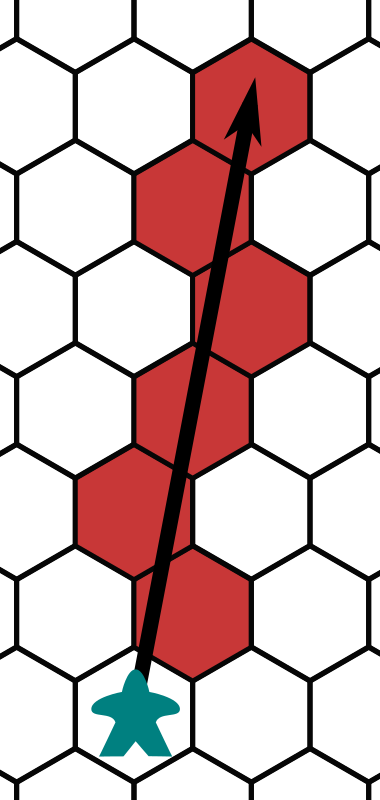
\includegraphics{graphics/throwing-cropped.png}
    \caption{A straight line approximated.}
    \label{fig:line-throw}
\end{figure}

\subsubsection{Failing a Throw}
If you fail a throw, roll a d6 and a fate die.
The d6 determines the distance it’s thrown, and the fate die determines how the throw diverges from the intended target.

Where the flag lands is determined in 2 steps:
\begin{enumerate}
    \item The Fate Die determines divergence
    \begin{enumerate}
        \item If you roll a +, the flag will fly towards the hex directly right of your intended target.
        \item If you roll a –, the flag will fly towards the hex directly left of your intended target.
        \item If you roll blank, the flag will not diverge from its intended target.
    \end{enumerate}
    \item The D6 is multiplied by 2 and determines distance.
    \begin{enumerate}
        \item If you roll a 1, the flag lands 2 hexes in front of the thrower.
        \item And if you roll 6, the flag lands 12 hexes away.
    \end{enumerate}
\end{enumerate}

\subsubsection{Chaining Throws}
Throws can also be chained.
If the character you're throwing the flag to hasn't acted yet, that character may throw the flag further.
This can be chained until you're out of usable characters.
\subsection{Passing}
Passing is the same as a throw, except the character you pass the flag to must be up to one hex away with nobody blocking the way.
Unlike throwing, passing cannot be intercepted.
\subsubsection{Failing a Pass}
If you fail a pass you roll a d6 and a fate die much like when you fail a throw.
However, because you’re passing a short distance, the d6 result is halved (rounded up), rather than doubled.
\subsection{Catching}
If you throw or pass the flag to someone, the flag must be caught.
Catching a flag requires rolling against Dex; a success means catching the flag, a fail means the recipient is knocked out (see Section~\ref{sec:knockout}), you then roll a d6 to determine in which hex around the recipient the flag lands.

\subsection{Getting Attacked}
If your character is attacked while holding a flag, the following happens:
\begin{description}
\item[Knocked Down] If your character is knocked down, the opponent gets to take the flag.
This does not apply to the Heavy, it is simply dropped instead, and you roll a d6 to see where it lands.
\item[Pushed] If your character is pushed, the opponent does not get the flag, it is merely pushed along.
\end{description}

\subsection{Dropping the Flag}
You can drop a flag as part of a regular move action.
You simply leave it where it is and continue moving.

\subsection{Out of Bounds}
If a player throws a flag out of bounds---out of the playing field---the previous player gets to place the flag on a hex of their choice in the middle zone.